%\nocite{1a21f4c7}
%\nocite{642a16a4}
%\nocite{ad05eef9}
%\nocite{c75138fd}
%\nocite{8b5861fc}
%\nocite{wiki-map00000}
%%%
In the final section of these preliminaries we discuss the concept of orientation of manifolds. Some proofs here are a bit technical and may be skipped if one is not interested in the technical details.
\\\\
We begin with a recap of what it means for a topological space to be a manifold, just to make clear which standards and notations we use. A second countable\footnote{second-countability is not always demanded for manifolds whereas the Hausdorff property is only rarely omitted; we require both here though the former is not needed for the results in this orientation section; however, the two properties imply the paracompactness of the manifold and manifolds that are not paracompact often behave a bit pathological as they generally do not enjoy some good/desired properties; paracompactness is somewhat weaker than second-countability, but additionally demanding that there are only countably many connected components is equivalent for manifolds} Hausdorff space $M$ is said to be an \textbf{$n$-dimensional manifold}, $n \in \mathbb{N}$, or shorter \textbf{$n$-manifold} if any point $x \in M$ has an open neighbourhood that is homeomorphic to an open subset of $\mathbb{R}^{n}$. A homeomorphism $\varphi \colon U \to O$ with $U \subset M$ open and containing $x$ and $O \subset \mathbb{R}^{n}$ open is called a \textbf{chart on $M$ (around $x$)}, often also written as a pair $(U,\varphi)$. We say that two charts $(U_{1},\varphi_{1})$ and $(U_{2},\varphi_{2})$ are \textbf{$C^{r}$-compatible}, $r \in \mathbb{N} \cup \lbrace \infty \rbrace$, if either $U_{1} \cap U_{2} = \emptyset$ or if the composition
\begin{align*}
  \varphi_{1}
  \circ
  \varphi_{2}^{-1}
  &\colon
  \varphi_{2}(U_{1} \cap U_{2})
  \to
  \varphi_{1}(U_{1} \cap U_{2})
\end{align*}
is a $C^{r}$-diffeomorphism. Such compositions are called \textbf{transition maps}. A set of pairwise $C^{r}$-compatible charts which covers $M$,
\begin{align*}
  \mathcal{A}
  &=
  \lbrace
    (U_{j},\varphi_{j})
    \colon
    j
    \in
    \mathsf{J}
  \rbrace
  \quad
  \text{with}
  \quad
  \bigcup_{j \in \mathsf{J}}
  U_{j}
  =
  M
\end{align*}
is a \textbf{$C^{r}$-atlas}. A subset of a $C^{r}$-atlas which is again a $C^{r}$-atlas is called a \textbf{subatlas}. Two $C^{r}$-atlases $\mathcal{A}_{1},\mathcal{A}_{2}$ are defined to be \textbf{$C^{r}$-equivalent} if their union $\mathcal{A}_{1} \cup \mathcal{A}_{2}$ is a $C^{r}$-atlas. The union of all atlases in an equivalence class is called a \textbf{maximal $C^{r}$-atlas}. A pair\footnote{we will mostly suppress $\mathcal{D}$ in the notation} $M \doteq (M,\mathcal{D})$ consisting of a manifold $M$ and an equivalence class of $C^{r}$-atlases $\mathcal{D}$ (or equivalently a maximal $C^{r}$-atlas) is a \textbf{$C^{r}$-manifold} and $\mathcal{D}$ is also called \textbf{$C^{r}$-structure}. We consider some special cases of regularity. In the case $r = 1$ we will mostly say \textbf{differentiable manifold} and \textbf{differentiable structure} and in the case $r = \infty$ we will usually use the adjective \textbf{smooth}. If $r = 0$, compatibility of charts is always satisfied of course and then a manifold will also be called \textbf{topological}. Note that in this last case there is only one maximal atlas consisting of all possible charts. Note further that for $s \leq r$ a $C^{r}$-structure gives rise to a $C^{s}$-structure by taking the maximal $C^{s}$-atlas containing the given maximal $C^{r}$-atlas.
\\
\begin{exa}
\label{exa:mfld}
Any open subset $O \subset \mathbb{R}^{n}$ is of course a smooth $n$-manifold itself since one can choose the $C^{\infty}$-structure containing the identity as a chart. In fact, for $n \neq 4$ there is an essentially unique smooth structure on $\mathbb{R}^{n}$, yet for $\mathbb{R}^{4}$ there are uncountably many different smooth structures.
\end{exa}
\begin{prf}
The first statement is clear. We will not elaborate on the second statement but the interested reader can search for exotic $\mathbb{R}^{4}$.
\\
\phantom{proven}
\hfill
$\Box$
\end{prf}
Unless stated otherwise we will always assume that the structure containing the identity is used when considering an open subset of $\mathbb{R}^{n}$ as a $C^{r}$-manifold.
\\
There are different ways to obtain a new manifold from a given one and we will only mention a few. For an open subset $A \subset M$ a $C^{r}$-structure on $M$ induces one on $A$ by restriction and we call $A$ with that structure an \textbf{open submanifold (of $M$)}. Moreover, we can form the cartesian product of manifolds by using the product atlas, yielding a manifold whose dimension is the sum of the dimensions of the component manifolds. We can also form the disjoint union of manifolds with the same dimension with the obvious atlas. Note however that the disjoint union of two manifolds of different dimension is not a manifold in our sense\footnote{it is possible to define manifolds with different dimensions on different connected components}.
\\
A map $f \colon M_{1} \to M_{2}$ between $C^{r}$-manifolds is said to be $C^{p}$, $p \leq r$, if for each $x \in M_{1}$ and chart $(U_{2},\varphi_{2})$ in the $C^{r}$-structure of $M_{2}$ with $f(x) \in U_{2}$, there is a chart $(U_{1},\varphi_{1})$ around $x$ in the $C^{r}$-structure of $M_{1}$ with $f(U_{1}) \subset U_{2}$ such that
\begin{align*}
  \varphi_{2}
  \circ
  f
  \circ
  \varphi_{1}^{-1}
  \colon
  \varphi_{1}(U_{1})
  &\to
  \varphi_{2}(U_{2})
\end{align*}
is $C^{p}$. If such an $f$ is bijective and $f^{-1}$ is $C^{p}$ as well then we call $f$ a \textbf{$C^{p}$-diffeomorphism}. If there is a $C^{1}$-diffeomorphism between $C^{r}$-manifolds then they are said to be \textbf{diffeomorphic}. In fact, the $C^{r}$-manifolds are the objects of a category $\mathbf{Diff}_{r}$ whose morphisms are $C^{r}$-maps. Note that this category admits finite products (the cartesian product) but the disjoint union does not serve as coproduct in general, whereas the full subcategory $\mathbf{Diff}_{r}^{n}$ with $C^{r}$-manifolds of a fixed dimension $n \in \mathbb{N}$ allows for finite coproducts (the disjoint union) but the cartesian product cannot be defined as the product of the category. Note that the empty set $\emptyset$ can be viewed as a manifold of any dimension and arbitrary regularity, that is, it is an object in every of the above categories.
\\
Finally, for $r \geq 1$ any $C^{r}$-structure contains a $C^{\infty}$-structure and any two $C^{\infty}$-structures contained in the $C^{r}$-structure are smoothly diffeomorphic. Thus a $C^{r}$-manifold can always be made into a smooth manifold in an essentially unique way, i.e. the way is unique up to diffeomorphism. However, $C^{p}$-maps do not become smooth when making the manifolds smooth so that there are still meaningful differences for different $p$ here.
\\\\
Next, we recall the definition of manifolds with boundary. For $n \geq 1$ a second-countable Hausdorff space $M$ is called an \textbf{$n$-manifold with boundary} if any point $x \in M$ has an open neighbourhood that is homeomorphic to an open subset of the half-space
\begin{align*}
  \mathbb{R}_{+}^{n}
  &:=
  \mathbb{R}^{n-1}
  \times
  [0,\infty)
\end{align*}
carrying the subspace topology as usual. A \textbf{chart with boundary (around $x$)} is a homeomorphism $\varphi \colon U \to O$ with $U \subset M$ open and containing $x$ and $O \subset \mathbb{R}_{+}^{n}$ open, often written as a pair $(U,\varphi)$.
\\
We say that a map
\begin{align*}
  f
  \colon
  S
  &\to
  \mathbb{R}^{m}
  ,\qquad
  m
  \in
  \mathbb{N}
\end{align*}
on a subset $S \subset \mathbb{R}_{+}^{n}$ is $C^{p}$ if there is an open set $\tilde{S} \subset \mathbb{R}^{n}$ with $S \subset \tilde{S}$ and a $C^{p}$-function $\tilde{f} \colon \tilde{S} \to \mathbb{R}^{m}$ such that
\begin{align*}
  \tilde{f}\vert S
  &=
  f
\end{align*}
For $m=n$ we call $f \colon S \to f(S)$ a \textbf{$C^{p}$-diffeomorphism} if $f$ is bijective and both $f$ and $f^{-1}$ are $C^{p}$. With this notion of differentiablility for the half space the notions $C^{r}$-compatibility, $C^{r}$-atlases, $C^{r}$-structure and hence \textbf{$C^{r}$-manifold with boundary} can be defined as for manifolds without boundary. Letting
\begin{align*}
  \lbrace
    (U_{j},\varphi_{j})
    \colon
    j
    \in
    \mathsf{J}
  \rbrace
\end{align*}
an atlas for $M$, the \textbf{boundary (of $M$)}\footnote{this is not to be confused with the topological boundary, which is always relative to a surrounding space; but here we consider abstract manifolds not embedded in a space so that the meaning should always be clear from the context; yet in fact it is true that $\partial M$ is the topological boundary of $\mathrm{int}(M)$ in $M$} is defined as
\begin{align*}
  \partial M
  :=
  \bigcup_{j \in \mathsf{J}}
  \varphi_{j}^{-1}
  \left(
    \varphi_{j}(U_{j})
    \cap
    \partial \mathbb{R}_{+}^{n}
  \right)
\end{align*}
where
\begin{align*}
  \partial
  \mathbb{R}_{+}^{n}
  &:=
  \lbrace
    (x_{1},\ldots,x_{n})
    \in
    \mathbb{R}^{n}
    \colon
    x_{n}
    =
    0
  \rbrace
\end{align*}
This is independent of the atlas chosen in the maximal atlas of $M$. Moreover, we define the \textbf{interior (of $M$)} to be
\begin{align*}
  \mathrm{int}(M)
  &:=
  M
  -
  \partial M
\end{align*}
By restricting charts it follows easily that $\mathrm{int}(M)$ is an $n$-manifold without boundary and $\partial M$ is an $(n-1)$-manifold without boundary and a diffeomorphism between manifolds with boundaries induces diffeomorphisms between the interiors and the boundaries.
\\
\begin{exa}
\label{exa:mfldwbd}
\begin{enumerate}
\item[(a)]
As for manifolds without boundary, any open subset $O \subset \mathbb{R}_{+}^{n}$ is a smooth $n$-manifold with boundary itself since one can choose the $C^{\infty}$-structure containing the identity as a chart.

\item[(b)]
Another example for a smooth $1$-dimensional manifold with boundary is the interval $[0,1]$ with smooth structure the maximal atlas containing the atlas consisting of the charts
\begin{align*}
  \mathrm{id}_{[0,1)}
  \qquad
  \text{and}
  \qquad
  \varphi
  \colon
  (0,1]
  &\to
  [0,1)
  ,\quad
  x
  \mapsto
  1 - x
\end{align*}
The boundary is
\begin{align*}
  \partial[0,1]
  &=
  \lbrace
    0,1
  \rbrace
\end{align*}
\end{enumerate}
\end{exa}
\begin{prf}
This is clear.
\\
\phantom{proven}
\hfill
$\Box$
\end{prf}
Note that a manifold without boundary can be viewed as a manifold with boundary whose boundary is empty. A manifold without boundary which is compact is also called \textbf{closed}. The $C^{r}$-manifolds with boundary together with the $C^{r}$-maps between them again form a category which we call $\mathbf{Diffb}_{r}$. For this category one can in general not take the cartesian product with the product atlas to be the product as this might lead to corners. For example, consider $[0,1] \times [0,1]$ with the smooth structure for $[0,1]$ from example \ref{exa:mfldwbd} above. Then the image of $\mathrm{id}_{[0,1)} \times \mathrm{id}_{[0,1)}$ is not an open subset of $\mathbb{R}_{+}^{2}$. Yet in the case of a manifold $M$ with empty boundary the cartesian product with any other manifold $B$ with boundary $\partial B$ is again a manifold whose boundary is $M \times \partial B$. If we fix the dimension $n \in \mathbb{N}$ then the resulting category $\mathbf{Diffb}_{r}^{n}$ again allows for finite coproducts using the disjoint union just as in the case of manifolds without boundary.
\\\\
As we use tangent spaces to define orientations of manifolds we recall some basics. Let $M$ be a $C^{r}$-manifold with boundary for $r \geq 1$. The \textbf{tangent space to $M$ at $x$}, denoted $T_{x}M$, is given by the set of equivalence classes of $C^{r}$-curves\footnote{there are other, equivalent ways of defining the tangent space like derivations or germs of smooth functions, but we restrict to the given one} at $x$, i.e. $C^{r}$-maps $c \colon I \to M$ where $I \subset \mathbb{R}$ is an interval with $0 \in I$ and $c(0) = x$. Here two such curves $c_{1},c_{2}$ are equivalent if for one - and thus each - chart $(U,\varphi)$ in the given structure with $x \in U$ we have
\begin{align*}
  \partial_{t}
  (\varphi \circ c_{1})(0)
  &=
  \partial_{t}
  (\varphi \circ c_{2})(0)
\end{align*}
Each chart $(U,\varphi)$ in the given atlas with $x \in U$ gives rise to the bijection
\begin{align*}
  T_{x}\varphi
  \colon
  T_{x}M
  \to
  \mathbb{R}^{n}
  ,\qquad
  [c]_{x}
  &\mapsto
  \partial_{t}
  (\varphi \circ c)(0)
\end{align*}
This bijection endows the tangent space $T_{x}M$ with the structure of an $n$-dimensional vector space and this vector space structure is independent of the chart. Hence $T_{x}\varphi$ is an isomorphism of vector spaces. If the manifold has no boundary one can restrict to open $I$ but for manifolds with boundary this is not sufficient since then the tangent space for a boundary point would be a vector space of lower dimension.
\\
The \textbf{tangent bundle of $M$} is
\begin{align*}
  TM
  &:=
  \bigcup_{x \in M}
  \lbrace
    x
  \rbrace
  \times
  T_{x}M
\end{align*}
Write
\begin{align*}
  \pi
  \colon
  TM
  &\to
  M
  ,\qquad
  (x,v)
  \mapsto
  x
\end{align*}
for the projection to the first coordinate. The tangent bundle can be given a topology and made into a $C^{r-1}$-manifold of dimension $2n$ using the charts of $M$. For a chart $\varphi \colon U \to O$ of $M$ the isomorphism $T_{x}\varphi$ yields a basis
\begin{align*}
  \left(
    b_{1}(x)
    ,
    \ldots
    ,
    b_{n}(x)
  \right)
  ,\qquad
  b_{i}(x)
  &:=
  (T_{x}\varphi)^{-1}(e_{i})
\end{align*}
of the vector space $T_{x}M$ for any $x \in U$ from the standard basis $(e_{1},\ldots,e_{n})$ of $\mathbb{R}^{n}$. Then the map\footnote{we use the Einstein summation convention}
\begin{align*}
  \Phi
  \colon
  \pi^{-1}(U)
  &\to
  O
  \times
  \mathbb{R}^{n}
  ,\qquad
  \left(
    x
    ,
    v^{i}
    b_{i}(x)
  \right)
  \mapsto
  \left(
    \varphi(x)
    ,
    v^{1}
    ,
    \ldots
    ,
    v^{n}
  \right)
\end{align*}
is a bijection. We take for all such charts of $M$ the sets of the form $\Phi^{-1}(V)$ for $V \subset O \times \mathbb{R}^{n}$ open as a basis for the topology on $TM$. The pairs $(\pi^{-1}(U),\Phi)$ then become the charts of a $C^{r-1}$-atlas of $TM$. The projection $\pi$ is then a $C^{r-1}$-map. Moreover, with the maps
\begin{align*}
  \phi
  \colon
  \pi^{-1}(U)
  &\to
  U
  \times
  \mathbb{R}^{n}
  ,\qquad
  \left(
    x
    ,
    v^{i}
    b_{i}(x)
  \right)
  \mapsto
  \left(
    x
    ,
    v^{1}
    ,
    \ldots
    ,
    v^{n}
  \right)
\end{align*}
as inverses of local trivializations, the tangent bundle $TM$ becomes an $n$-dimensional real $C^{r-1}$-vector bundle over $M$. Note that for another chart $(\hat{\varphi},\hat{U})$ of $M$ the transition function of this vector bundle for $\phi^{-1}$ and $\hat{\phi}^{-1}$ is
\begin{align*}
  g_{U,\hat{U}}
  \colon
  U
  \cap
  \hat{U}
  &\to
  GL(n)
  ,\qquad
  x
  \mapsto
  T_{x}\varphi
  \circ
  (T_{x}\hat{\varphi})^{-1}
\end{align*}
For a $C^{r}$-map $f \colon M_{1} \to M_{2}$ between two manifolds with boundary the \textbf{differential} between the tangent bundles is
\begin{align*}
  Tf
  \colon
  TM_{1}
  \to
  TM_{2}
  ,\qquad
  (x,[c]_{x})
  &\mapsto
  (f(x),[f \circ c]_{f(x)})
\end{align*}
or shorter (abusing notation)
\begin{align*}
  Tf([c]_{x})
  &:=
  [f \circ c]_{f(x)}
\end{align*}
The restriction to a tangent space at a point $x \in M_{1}$ is written
\begin{align*}
  T_{x}f
  \colon
  T_{x}M_{1}
  &\to
  T_{f(x)}M_{2}
\end{align*}
Forming tangent bundles of $C^{r}$-manifolds and differentials of $C^{r}$-maps makes up a functor called $T$ from $\mathbf{Diffb}_{r}$ to the category of real $C^{r-1}$-vector bundles. This means that
\begin{align*}
  T(f_{2} \circ f_{1})
  &=
  Tf_{2}
  \circ
  Tf_{1}
\end{align*}
for
\begin{align*}
  f_{1}
  \in
  \mathrm{mor}_{\mathbf{Diffb}_{r}}(M_{1},M_{2})
  \qquad
  \text{and}
  \qquad
  f_{2}
  \in
  \mathrm{mor}_{\mathbf{Diffb}_{r}}(M_{2},M_{3})
\end{align*}
and
\begin{align*}
  T\mathrm{id}_{M}
  &=
  \mathrm{id}_{TM}
\end{align*}
for $M \in \mathrm{ob}_{\mathbf{Diffb_{r}}}$. Note that when we canonically identify $T_{x}M$ with $T_{x}U$ and $T_{\varphi(x)}O$ with $\mathbb{R}^{n}$ for a chart $\varphi \colon U \to O$, which we will keep doing implicitly from now on, then the differential of the chart at a point is nothing but the isomorphism of vector spaces defined above,
\begin{align*}
  T_{x}\varphi
  \colon
  T_{x}M
  \cong
  T_{x}U
  &\to
  T_{\varphi(x)}O
  \cong
  \mathbb{R}^{n}
\end{align*}
\\
Now let us get to orientations of manifolds. We first consider the empty manifold. Here the concept of orientation does not make much sense since there is nothing to assign an orientation to. For convenience we thus stipulate that the empty manifold is orientable and has precisely one orientation. For the rest of this section we assume a manifold to be non-empty unless stated otherwise. Next, consider the easy special case of a zero-dimensional manifold $M$ which is basically just a collection of points. Here an \textbf{orientation} is just a function
\begin{align*}
  \sigma
  \colon
  M
  &\to
  \lbrace
    -1
    ,
    +1
  \rbrace
\end{align*}
A bijection between two oriented zero-dimensional manifolds is then of course \textbf{orientation-preserving} if it maps points with orientation $+1$ to points with orientation $+1$ and likewise for the points with orientation $-1$.
\\
For higher dimensions there are several somewhat different definitions of orientability for manifolds. We will not dicuss all of them here. Some of the definitions require a differentiable structure, but there are also definitions which do not, making use of some homology instead. We start with the differentiable case, which allows for a probably more intuitive definition in terms of the tangent spaces which are finite-dimensional vector spaces. Recall that an orientation of such a vector space $V$ can be defined as one of the two equivalence classes of ordered bases where two ordered bases are equivalent - or have the same orientation - if the unique linear map transforming one ordered basis into the other has positive determinant. We will write $[\mathcal{B}]_{V}$ for such an orientation where $\mathcal{B}$ is an ordered basis of $V$ representing the orientation and we let $\mathrm{Or}_{V}$ denote the set of the two different orientations of $V$. Then, given two finite-dimensional vector spaces $V_{1},V_{2}$ with orientations $[\mathcal{B}_{1}]_{V_{1}},[\mathcal{B}_{2}]_{V_{2}}$, a linear isomorphism $L \colon V_{1} \to V_{2}$ between them is orientation-preserving, if it maps one, and thus each\footnote{this is clear since for an automorphism $\varphi$ on $V_{1}$ we obtain an automorphism $L \circ \varphi \circ L^{-1}$ on $V_{2}$ with the same determinant}, ordered basis in $[\mathcal{B}_{1}]_{V_{1}}$ to an ordered basis in $[\mathcal{B}_{2}]_{V_{2}}$. Else it is orientation-reversing. Note that in the case that $V_{2} = V_{1}$ this amounts to demanding that $L$ has positive or negative determinant, respectivley. Note further that if the other orientation is chosen for one of the vector spaces then an orientation-preserving isomorphism becomes orientation-reversing and vice versa.
\\
Now we define a \textbf{tangential orientation} for a differentiable $n$-manifold $M$ without boundary, $n \in \mathbb{N}^{\times}$, to be a \textbf{consistent choice} of orientations of the tangent spaces $T_{x}M$ at each $x \in M$, which is a map
\begin{align*}
  \mathfrak{C}
  \colon
  M
  &\to
  \bigcup_{x \in M}
  \mathrm{Or}_{T_{x}M}
\end{align*}
such that $\mathfrak{C}(x) \in \mathrm{Or}_{T_{x}M}$ and such that there is a subatlas of the differentiable structure of $M$ with the property that for every point $x \in M$ and any chart $(U,\varphi)$ around $x$ the differential
\begin{align*}
  T_{y}\varphi
  \colon
  T_{y}M
  &\to
  \mathbb{R}^{n}
\end{align*}
is orientation-preserving for all $y \in U$, where we fix the standard orientation on $\mathbb{R}^{n}$, i.e. the one coming from the standard basis. We call $M$ \textbf{tangentially orientable} if such a tangential orientation exists and a manifold together with a tangential orientation is a \textbf{tangentially oriented manifold}, where we will mostly leave the orientation implicit in the notation.
\\
It is clear that a tangential orientation of $M$ induces one on every open submanifold. A $C^{1}$-diffeomorphism $f \colon M_{1} \to M_{2}$ between two tangentially oriented manifolds without boundary is defined to be \textbf{tangentially orientation-preserving} if the linear isomorphism
\begin{align*}
  T_{x}f
  \colon
  T_{x}M_{1}
  &\to
  T_{f(x)}M_{2}
\end{align*}
is orientation-preserving for every $x \in M_{1}$.
\\
\begin{exa}
\label{exa:orientation}
\begin{enumerate}
\item[(a)]
We illsutrate the idea that is captured by this definition of orientation for the circle $S^{1}$ which is tangentially orientable. Intuitively an orientation for a manifold is such that the orientation of the tangent space is not reversed from one point to a neighboured point. As the tangent spaces of the circle are $1$-dimensional an orientation basically is a direction tangent to the circle at every point in such a way that the direction is not reversed when going to the next point. Thus figure \ref{fig:orcirc} illustrates an orientation for the circle whereas figure \ref{fig:norcirc} does not.
\\
\begin{figure}[h!]
\centering
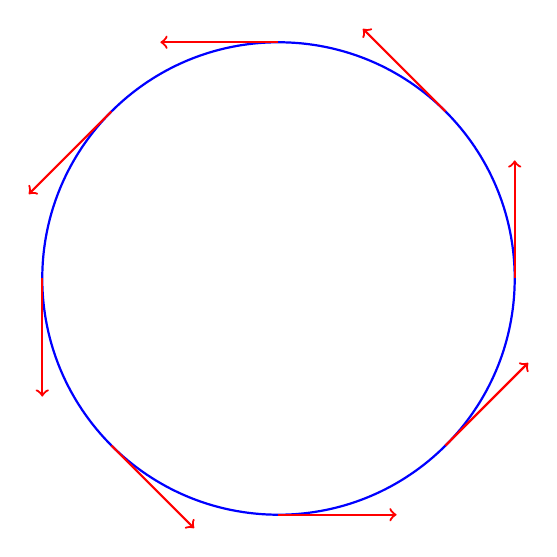
\begin{tikzpicture}[scale=3,thick]
  %circle
  \draw[blue] circle (1cm);

  %arrows
  \draw[red,->] (0:1) -- +(0,0.5);
  \draw[red,->] (45:1) -- +(-0.35,0.35);
  \draw[red,->] (90:1) -- +(-0.5,0);
  \draw[red,->] (135:1) -- +(-0.35,-0.35);
  \draw[red,->] (180:1) -- +(0,-0.5);
  \draw[red,->] (225:1) -- +(0.35,-0.35);
  \draw[red,->] (270:1) -- +(0.5,0);
  \draw[red,->] (315:1) -- +(0.35,0.35);
\end{tikzpicture}
\caption{Orientation for the circle}
\label{fig:orcirc}
\end{figure}
\\
\begin{figure}[h!]
\centering
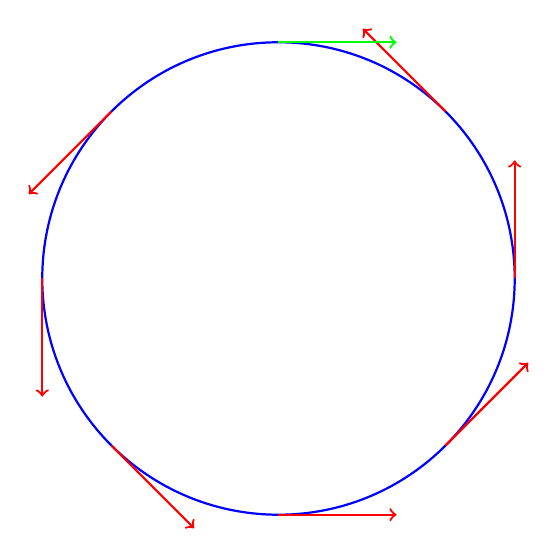
\begin{tikzpicture}[scale=3,thick]
  %circle
  \draw[blue] circle (1cm);

  %arrows
  \draw[red,->] (0:1) -- +(0,0.5);
  \draw[red,->] (45:1) -- +(-0.35,0.35);
  \draw[green,->] (90:1) -- +(0.5,0);
  \draw[red,->] (135:1) -- +(-0.35,-0.35);
  \draw[red,->] (180:1) -- +(0,-0.5);
  \draw[red,->] (225:1) -- +(0.35,-0.35);
  \draw[red,->] (270:1) -- +(0.5,0);
  \draw[red,->] (315:1) -- +(0.35,0.35);
\end{tikzpicture}
\caption{Not an orientation for the circle}
\label{fig:norcirc}
\end{figure}
\\

\item[(b)]
The standard example for a tangentially non-orientable manifold is the open M{\"o}bius strip which can be given by identifying the top and the bottom of the square in the opposite direction, i.e.
\begin{align*}
  (0,1)
  \times
  [0,1]
  \qquad
  \text{with}
  \qquad
  (x_{1},0)
  \sim
  (1-x_{1},1)
  \quad
  \text{for }
  x_{1}
  \in
  (0,1)
\end{align*}
as depicted in figure \ref{fig:moebius}. This means that the square is twisted once before the top and bottom edge are glued together. An orientation would be a consistent choice of a $2$-dimensional basis for the tangent space at each point but the twist basically reverses one direction of this basis without changing the other, thus reversing the whole orientation at the top/bottom edge as illustrated in figure \ref{fig:moebius}.
\\
%/*
%\iffalse
\begin{figure}[h!]
\centering
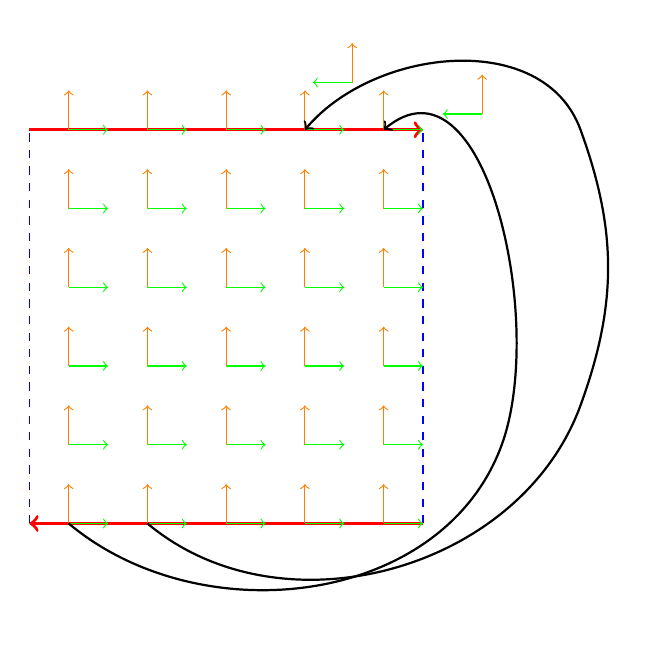
\begin{tikzpicture}[scale=5,thick]
  %rectangle
  \draw[blue,thin,dashed] (0,0) -- (0,1);
  \draw[red,very thick,->] (0,1) -- (1,1);
  \draw[blue,thin,dashed] (1,0) -- (1,1);
  \draw[red,very thick,->] (1,0) -- (0,0);

  %orientations
  %left
  \draw[green,->,thin] (0.1,0) -- +(0.1,0);
  \draw[orange,->,thin] (0.1,0) -- +(0,0.1);
  \draw[green,->,thin] (0.1,0.2) -- +(0.1,0);
  \draw[orange,->,thin] (0.1,0.2) -- +(0,0.1);
  \draw[green,->,thin] (0.1,0.4) -- +(0.1,0);
  \draw[orange,->,thin] (0.1,0.4) -- +(0,0.1);
  \draw[green,->,thin] (0.1,0.6) -- +(0.1,0);
  \draw[orange,->,thin] (0.1,0.6) -- +(0,0.1);
  \draw[green,->,thin] (0.1,0.8) -- +(0.1,0);
  \draw[orange,->,thin] (0.1,0.8) -- +(0,0.1);
  \draw[green,->,thin] (0.1,1) -- +(0.1,0);
  \draw[orange,->,thin] (0.1,1) -- +(0,0.1);
  %left-middle
  \draw[green,->,thin] (0.3,0) -- +(0.1,0);
  \draw[orange,->,thin] (0.3,0) -- +(0,0.1);
  \draw[green,->,thin] (0.3,0.2) -- +(0.1,0);
  \draw[orange,->,thin] (0.3,0.2) -- +(0,0.1);
  \draw[green,->,thin] (0.3,0.4) -- +(0.1,0);
  \draw[orange,->,thin] (0.3,0.4) -- +(0,0.1);
  \draw[green,->,thin] (0.3,0.6) -- +(0.1,0);
  \draw[orange,->,thin] (0.3,0.6) -- +(0,0.1);
  \draw[green,->,thin] (0.3,0.8) -- +(0.1,0);
  \draw[orange,->,thin] (0.3,0.8) -- +(0,0.1);
  \draw[green,->,thin] (0.3,1) -- +(0.1,0);
  \draw[orange,->,thin] (0.3,1) -- +(0,0.1);
  %middle
  \draw[green,->,thin] (0.5,0) -- +(0.1,0);
  \draw[orange,->,thin] (0.5,0) -- +(0,0.1);
  \draw[green,->,thin] (0.5,0.2) -- +(0.1,0);
  \draw[orange,->,thin] (0.5,0.2) -- +(0,0.1);
  \draw[green,->,thin] (0.5,0.4) -- +(0.1,0);
  \draw[orange,->,thin] (0.5,0.4) -- +(0,0.1);
  \draw[green,->,thin] (0.5,0.6) -- +(0.1,0);
  \draw[orange,->,thin] (0.5,0.6) -- +(0,0.1);
  \draw[green,->,thin] (0.5,0.8) -- +(0.1,0);
  \draw[orange,->,thin] (0.5,0.8) -- +(0,0.1);
  \draw[green,->,thin] (0.5,1) -- +(0.1,0);
  \draw[orange,->,thin] (0.5,1) -- +(0,0.1);
  %right-middle
  \draw[green,->,thin] (0.7,0) -- +(0.1,0);
  \draw[orange,->,thin] (0.7,0) -- +(0,0.1);
  \draw[green,->,thin] (0.7,0.2) -- +(0.1,0);
  \draw[orange,->,thin] (0.7,0.2) -- +(0,0.1);
  \draw[green,->,thin] (0.7,0.4) -- +(0.1,0);
  \draw[orange,->,thin] (0.7,0.4) -- +(0,0.1);
  \draw[green,->,thin] (0.7,0.6) -- +(0.1,0);
  \draw[orange,->,thin] (0.7,0.6) -- +(0,0.1);
  \draw[green,->,thin] (0.7,0.8) -- +(0.1,0);
  \draw[orange,->,thin] (0.7,0.8) -- +(0,0.1);
  \draw[green,->,thin] (0.7,1) -- +(0.1,0);
  \draw[orange,->,thin] (0.7,1) -- +(0,0.1);
  %right
  \draw[green,->,thin] (0.9,0) -- +(0.1,0);
  \draw[orange,->,thin] (0.9,0) -- +(0,0.1);
  \draw[green,->,thin] (0.9,0.2) -- +(0.1,0);
  \draw[orange,->,thin] (0.9,0.2) -- +(0,0.1);
  \draw[green,->,thin] (0.9,0.4) -- +(0.1,0);
  \draw[orange,->,thin] (0.9,0.4) -- +(0,0.1);
  \draw[green,->,thin] (0.9,0.6) -- +(0.1,0);
  \draw[orange,->,thin] (0.9,0.6) -- +(0,0.1);
  \draw[green,->,thin] (0.9,0.8) -- +(0.1,0);
  \draw[orange,->,thin] (0.9,0.8) -- +(0,0.1);
  \draw[green,->,thin] (0.9,1) -- +(0.1,0);
  \draw[orange,->,thin] (0.9,1) -- +(0,0.1);

  %identification
  \draw[->] (0.1,0) to [out=-40,in=-110] (1.2,0.2) to [out=70,in=40] (0.9,1);
  \draw[green,->,thin] (1.15,1.04) -- +(-0.1,0);
  \draw[orange,->,thin] (1.15,1.04) -- +(0,0.1);
  \draw[->] (0.3,0) to [out=-40,in=-110] (1.4,0.3) to [out=70,in=-70] (1.4,1) to [out=110,in=50] (0.7,1);
  \draw[green,->,thin] (0.82,1.12) -- +(-0.1,0);
  \draw[orange,->,thin] (0.82,1.12) -- +(0,0.1);
\end{tikzpicture}
\caption{The open M{\"o}bius strip as non-orientable manifold}
\label{fig:moebius}
\end{figure}
%\fi
%*/
\end{enumerate}
\end{exa}
\begin{prf}
The technical details can be filled in as an exercise.
\\
\phantom{proven}
\hfill
$\Box$
\end{prf}
Let now $(U_{1},\varphi_{1}),(U_{2},\varphi_{2})$ be two charts belonging to a subatlas according to a tangential orientation of $M$, let $x \in U_{1} \cap U_{2}$ and let $(v_{1},\ldots,v_{n})$ be an ordered basis of $T_{x}M$. Then
\begin{align*}
  \left(
    T_{x}\varphi_{1}(v_{1})
    ,
    \ldots
    ,
    T_{x}\varphi_{1}(v_{n})
  \right)
  \qquad
  \text{and}
  \qquad
  \left(
    T_{x}\varphi_{2}(v_{1})
    ,
    \ldots
    ,
    T_{x}\varphi_{2}(v_{n})
  \right)
\end{align*}
belong to the same orientation on $\mathbb{R}^{n}$. Since
\begin{align*}
  T_{x}\varphi_{1}
  &=
  T_{\varphi_{2}(x)}(\varphi_{1} \circ \varphi_{2}^{-1})
  \circ
  T_{x}\varphi_{2}
\end{align*}
we can conclude that
\begin{align*}
  T_{\varphi_{2}(x)}
  \left(
    \varphi_{1}
    \circ
    \varphi_{2}^{-1}
  \right)
\end{align*}
is orientation-preserving for all $x \in U_{1} \cap U_{2}$, that is, the determinant of this linear map - which is nothing but the Jacobian determinant of the transition map $\varphi_{1} \circ \varphi_{2}^{-1}$ at $\varphi_{2}(x)$ - is positive for all $x \in U_{1} \cap U_{2}$. We call a $C^{1}$-diffeomorphism $f \colon O_{1} \to O_{2}$ between open subsets of $\mathbb{R}^{n}$ \textbf{differentiably standard orientation-preserving} if the Jacobian determinant of $f$ is positive at each point in $O_{1}$ and \textbf{differentiably standard orientation-reversing} if the Jacobian determinant is negative everywhere. Note that since the Jacobian determinant for such an $f$ is a continuous function from $O_{1}$ to $\mathbb{R} \setminus \lbrace 0 \rbrace$, its sign is constant if $O_{1}$ is connected. Now a differentiable atlas is called \textbf{differentiably oriented} if all transition maps are differentiably standard orientation-preserving. We say that $M$ is \textbf{differentiably orientable} if there exists a differentiably oriented atlas. A \textbf{differentiable orientation} is then a maximal differentiably oriented atlas, which means that this atlas is not properly contained in another differentiably oriented atlas\footnote{this notion of maximality can, of course, be equivalently defined as the union of all corresponding atlases in an equivalence class where two such atlases are equivalent if their union is again such an atlas}. A manifold together with a differentiable orientation is a \textbf{differentiably oriented manifold}.
\\
Of course, a differentiable orientation on an open submanifold is induced by restricting the charts of the differentiable orientation of $M$. This is because the chart obtained by restricting a chart in the maximal differentiably oriented atlas of $M$ to an open subset is again in that atlas. A $C^{1}$-diffeomorphism $f \colon M_{1} \to M_{2}$ between two differentiably oriented manifolds without boundary is defined to be \textbf{differentiably orientation-preserving} if for each chart $(U_{2},\varphi_{2})$ in the differentiable orientation of $M_{2}$ the chart
\begin{align*}
  \left(
    f^{-1}(U_{2})
    ,
    \varphi_{2}
    \circ
    f
  \right)
\end{align*}
is in the differentiable orientation of $M_{1}$.
\\
Note that in the language of the tangent bundle $TM$ a differentiable orientation is a (maximal) atlas of local trivializations such that the transition functions have only values in
\begin{align*}
  GL_{+}(n)
  \subset
  GL(n)
\end{align*}
But this is actually nothing but a reduction of the structure group of the tangent bundle to $GL_{+}(n)$, providing an equivalent definition for orientation.
\\
\begin{exa}
\label{exa:difforstdpr}
As an example consider open submanifolds $M_{1},M_{2}$ of $\mathbb{R}^{n}$ each equipped with a differentiable orientation and a $C^{1}$-diffeomorphism $f \colon M_{1} \to M_{2}$ such that for each of the corresponding connected components $C_{1} \subset M_{1}$ and $f(C_{1}) \subset M_{2}$ either $(C_{1},\mathrm{id}_{C_{1}})$ and $(f(C_{1}),\mathrm{id}_{f(C_{1})})$ belong to the respective differentiable orientations or neither of them does. Then the notion of a differentiably orientation-preserving $C^{1}$-diffeomorphism coincides with the notion of a differentiably standard orientation-preserving $C^{1}$-diffeomorphism.
\end{exa}
\begin{prf}[Sketch]
This is because if the identity chart for a connected component is contained in the differentiable orientation then all charts in that atlas (and their inverses) are transition maps and therefore differentiably standard orientation-preserving on that component. Else all the charts are differentiably standard orientation-reversing on that component. Then the claim follows because if both maps in a composition of $C^{1}$-diffeomorphisms between open subsets of $\mathbb{R}^{n}$ are differentiably standard orientation-preserving or -reversing then the composition is differentiably standard orientation-preserving and if one of them is differentiably standard orientation-preserving and the other is -reversing then the composition is differentiably standard orientation-reversing.
\\
\phantom{proven}
\hfill
$\Box$
\end{prf}
For the, a priori different, notions of tangential and differentiable orientation we have the following
\\
\begin{thm}
\label{thm:equivtangdiff}
A differentiable $n$-manifold without boundary $M$ is tangentially orientable if and only if it is differentiably orientable.
\end{thm}
\begin{prf}
From what was said before it is clear that a tangential orientation yields a differentiably oriented atlas and that the corresponding differentiable orientation is given by adding all charts to the atlas whose differentials are orientation-preserving at all points w.r.t. the given tangential orientation.
\\
Suppose now that we have a differentiable orientation on $M$. Then we can define an orientation of $T_{x}M$ for $x \in M$ by pulling back the standard orientation of $\mathbb{R}^{n}$ via a chart $(U_{1},\varphi_{1})$ around $x$. This means the orientation on $T_{x}M$ is chosen to be the one containing the basis
\begin{align*}
  \left(
    T_{\varphi_{1}(x)}
    \varphi_{1}^{-1}(e_{1})
    ,
    \ldots
    ,
    T_{\varphi_{1}(x)}
    \varphi_{1}^{-1}(e_{n})
  \right)
\end{align*}
where $(e_{1},\ldots,e_{n})$ is the standard basis of $\mathbb{R}^{n}$. With this orientation $T_{\varphi_{1}(x)}\varphi_{1}^{-1}$ and thus, of course, $T_{x}\varphi_{1}$ are orientation-preserving isomorphisms. For the well-definedness we have to check that the orientation does not depend on the chosen chart. Let $(U_{2},\varphi_{2})$ be another chart around $x$. We know that
\begin{align*}
  (e_{1},\ldots,e_{n})
  \qquad
  \text{and}
  \qquad
  \left(
    T_{\varphi_{2}(x)}(\varphi_{1} \circ \varphi_{2}^{-1})(e_{1})
    ,
    \ldots
    ,
    T_{\varphi_{2}(x)}(\varphi_{1} \circ \varphi_{2}^{-1})(e_{n})
  \right)
\end{align*}
belong to the same orientation of $\mathbb{R}^{n}$. Hence, by applying $T_{\varphi_{1}(x)}\varphi_{1}^{-1}$ we see that
\begin{align*}
  \left(
    T_{\varphi_{1}(x)}\varphi_{1}^{-1}(e_{1})
    ,
    \ldots
    ,
    T_{\varphi_{1}(x)}\varphi_{1}^{-1}(e_{n})
  \right)
  \qquad
  \text{and}
  \qquad
  \left(
    T_{\varphi_{2}(x)}\varphi_{2}^{-1}(e_{1})
    ,
    \ldots
    ,
    T_{\varphi_{2}(x)}\varphi_{2}^{-1}(e_{n})
  \right)
\end{align*}
belong to the same orientation of $T_{x}M$. This additionally shows that $T_{x}\varphi_{2}$ is orientation-preserving as well. Thus these induced orientations on the tangential spaces are a tangential orientation with the given maximal oriented atlas.
\\
\phantom{proven}
\hfill
$\Box$
\end{prf}
It is clear that the constructions in the above proof to obtain a differentiable orientation from a tangential orientation and vice versa are inverse to each other, i.e. applying them consecutively in either order yields the original orientation.
\\\\
The definition of orientability in terms of an oriented atlas makes perfect sense even without a differentiable structure, except for the notion of a differentiably standard orientation-preserving transition map as the transition maps are now merely homeomorphisms and not necessarily $C^{1}$-diffeomorphisms anymore. Thus we need a notion of what it means for a homeomorphism between open subsets of $\mathbb{R}^{n}$ to be orientation-preserving. For this purpose we make use of some singular homology and we will use the notation from the homology chapter in the appendix. So the reader who does not know the notions and symbols here should have a look at the appendix first.
\\
Let $f \colon O_{1} \to O_{2}$ a homeomorphism between open subsets of $\mathbb{R}^{n}$ and let $x \in O_{1}$. Then $f$ induces an isomorphism $f_{x}$ in $\mathbf{Top_{2}}$ between the ordered pairs
\begin{align*}
  (O_{1},O_{1} - \lbrace x \rbrace)
  \qquad
  \text{and}
  \qquad
  (O_{2},O_{2} - \lbrace f(x) \rbrace)
\end{align*}
and hence an isomorphism
\begin{align*}
  H_{n}(f_{x})
  \colon
  H_{n}
  \left(
    (O_{1},O_{1} - \lbrace x \rbrace)
  \right)
  &\to
  H_{n}
  \left(
    (O_{2},O_{2} - \lbrace f(x) \rbrace)
  \right)
\end{align*}
of singular homology groups. By excision, (HT3), we obtain an isomorphism
\begin{align*}
  H_{n}
  \left(
    i_{x,O_{1}}^{\mathbb{R}^{n}}
  \right)
  \colon
  H_{n}
  \left(
    (O_{1},O_{1} - \lbrace x \rbrace)
  \right)
  \to
  H_{n}
  \left(
    (\mathbb{R}^{n},\mathbb{R}^{n} - \lbrace x \rbrace)
  \right)
\end{align*}
induced by the inclusion
\begin{align*}
  i_{x,O_{1}}^{\mathbb{R}^{n}}
  \colon
  (O_{1},O_{1} - \lbrace x \rbrace)
  &\to
  (\mathbb{R}^{n},\mathbb{R}^{n} - \lbrace x \rbrace)
\end{align*}
since
\begin{align*}
  \overline{O_{1}^{c}}
  &=
  O_{1}^{c}
  \subset
  \mathbb{R}^{n}
  -
  \lbrace x \rbrace
\end{align*}
and $\mathbb{R}^{n} - \lbrace x \rbrace$ is open because $\mathbb{R}^{n}$ is Hausdorff and thus singleton sets are closed. Moreover, the translation map
\begin{align*}
  \tau_{x}
  \colon
  \mathbb{R}^{n}
  &\to
  \mathbb{R}^{n}
  ,\qquad
  y
  \mapsto
  y + x
\end{align*}
induces an isomorphism
\begin{align*}
  t_{x}
  \colon
  (\mathbb{R}^{n},\mathbb{R}^{n} - \lbrace 0 \rbrace)
  &\to
  (\mathbb{R}^{n},\mathbb{R}^{n} - \lbrace x \rbrace)
\end{align*}
in $\mathbf{Top_{2}}$ and thus $H_{n}(t_{x})$ is an isomorphism. Composition then yields an isomorphism
\begin{align*}
  \iota_{x,O_{1}}
  &:=
  H_{n}(t_{x}^{-1})
  \circ
  H_{n}(i_{x,O_{1}}^{\mathbb{R}^{n}})
  \colon
  H_{n}
  \left(
    (O_{1},O_{1} - \lbrace x \rbrace)
  \right)
  \to
  H_{n}
  \left(
    (\mathbb{R}^{n},\mathbb{R}^{n} - \lbrace 0 \rbrace)
  \right)
\end{align*}
Analogously, we obtain an isomorphism
\begin{align*}
  \iota_{f(x),O_{2}}
  &:=
  H_{n}(t_{f(x)}^{-1})
  \circ
  H_{n}(i_{f(x),O_{2}}^{\mathbb{R}^{n}})
  \colon
  H_{n}
  \left(
    (O_{2},O_{2} - \lbrace f(x) \rbrace)
  \right)
  \to
  H_{n}
  \left(
    (\mathbb{R}^{n},\mathbb{R}^{n} - \lbrace 0 \rbrace)
  \right)
\end{align*}
Using that $\mathbb{R}^{n}$ is contractible and that $\mathbb{R}^{n} - \lbrace 0 \rbrace$ is homotopy equivalent to the $(n-1)$-sphere $S^{n-1}$ it is not hard to see (cf. e.g. \cite{8b5861fc}) with the long exact sequence of homology groups that
\begin{align*}
  H_{n}((\mathbb{R}^{n},\mathbb{R}^{n} - \lbrace 0 \rbrace))
  &\cong
  \mathbb{Z}
\end{align*}
Hence we define $f$ to be \textbf{topologically standard orientation-preserving} if
\begin{align*}
  \iota_{f(x),O_{2}}
  \circ
  H_{n}(f_{x})
  \circ
  \iota_{x,O_{1}}^{-1}
  &=
  \mathrm{id}_{H_{n}((\mathbb{R}^{n},\mathbb{R}^{n} - \lbrace 0 \rbrace))}
\end{align*}
for each $x \in O_{1}$, that is if these maps all fix the two generators of $H_{n}((\mathbb{R}^{n},\mathbb{R}^{n} - \lbrace 0 \rbrace))$. If the generators are interchanged for all $x \in O_{1}$ we call $f$ \textbf{topologically standard orientation-reversing}. It will become clear later that if $O_{1}$ is connected then either all these maps fix the two generators or all these maps interchange the generators. An atlas of an $n$-manifold without boundary $M$ is then called \textbf{topologically oriented} if all transition maps are topologically standard orientation-preserving. We call $M$ \textbf{topologically orientable} if there exists a topologically oriented atlas. A \textbf{topological orientation} is then a maximal topologically oriented atlas and a manifold together with a topological orientation is a \textbf{topologically oriented manifold}.
\\
Note that for an open subset $\tilde{O}_{1} \subset O_{1}$ with $x \in \tilde{O}_{1}$ the inclusion
\begin{align*}
  i_{x,\tilde{O}_{1}}^{O_{1}}
  \colon
  (\tilde{O}_{1},\tilde{O}_{1} - \lbrace x \rbrace)
  &\to
  (O_{1},O_{1} - \lbrace x \rbrace)
\end{align*}
induces an isomorphism $H_{n}(i_{x,\tilde{O}_{1}}^{O_{1}})$ by excision, (HT3), because $O_{1} - \tilde{O}_{1}$ is closed in $O_{1}$. Analogously, we have an isomorphism induced by $i_{f(x),\tilde{O}_{2}}^{O_{2}}$ for $\tilde{O}_{2} := f(\tilde{O}_{1})$. Further note that
\begin{align*}
  i_{x,O_{1}}^{\mathbb{R}^{n}}
  \circ
  i_{x,\tilde{O}_{1}}^{O_{1}}
  &=
  i_{x,\tilde{O}_{1}}^{\mathbb{R}^{n}}
  \\
  i_{f(x),O_{2}}^{\mathbb{R}^{n}}
  \circ
  i_{f(x),\tilde{O}_{2}}^{O_{2}}
  &=
  i_{f(x),\tilde{O}_{2}}^{\mathbb{R}^{n}}
  \\
  f_{x}
  \circ
  i_{x,\tilde{O}_{1}}^{O_{1}}
  &=
  i_{f(x),\tilde{O}_{2}}^{O_{2}}
  \circ
  \tilde{f_{x}}
\end{align*}
where
\begin{align*}
  \tilde{f_{x}}
  &:=
  f_{x}
  \vert
  (\tilde{O}_{1},\tilde{O}_{1} - \lbrace x \rbrace)
\end{align*}
Applying $H_{n}$ to these equations and using the functoriality we obtain
\begin{align*}
  H_{n}(i_{x,O_{1}}^{\mathbb{R}^{n}})
  \circ
  H_{n}(i_{x,\tilde{O}_{1}}^{O_{1}})
  &=
  H_{n}(i_{x,\tilde{O}_{1}}^{\mathbb{R}^{n}})
  \\
  H_{n}(i_{f(x),O_{2}}^{\mathbb{R}^{n}})
  \circ
  H_{n}(i_{f(x),\tilde{O}_{2}}^{O_{2}})
  &=
  H_{n}(i_{f(x),\tilde{O}_{2}}^{\mathbb{R}^{n}})
  \\
  H_{n}(f_{x})
  \circ
  H_{n}(i_{x,\tilde{O}_{1}}^{O_{1}})
  &=
  H_{n}(i_{f(x),\tilde{O}_{2}}^{O_{2}})
  \circ
  H_{n}(\tilde{f_{x}})
\end{align*}
With these equations it is easy to see that
\begin{align*}
  \iota_{f(x),\tilde{O}_{2}}
  \circ
  H_{n}(\tilde{f_{x}})
  \circ
  \iota_{x,\tilde{O}_{1}}^{-1}
  &=
  \iota_{f(x),O_{2}}
  \circ
  H_{n}(f_{x})
  \circ
  \iota_{x,O_{1}}^{-1}
\end{align*}
which shows that restrictions of topologically standard orientation-preserving homeomorphisms to open subsets are again topologically standard orientation-preserving. It further shows that it suffices to find a topologically standard orientation-preserving restriction to an open neighbourhood for any point in $O_{1}$ to show that $f$ is topologically standard orientation-preserving. As any open set of $\mathbb{R}^{n}$, and more generally any manifold, is locally path-connected we know that any connected component is open. Thus it suffices in particular to show that $f$ is topologically standard orientation-preserving on each component.
\\
From this it is immediate that restrictions of charts of a topological orientation to open subsets are also in that topological orientation. Therefore we obtain a topological orientation on an open submanifold by restriction. Moreover, a homeomorphism $f \colon M_{1} \to M_{2}$ between two topologically oriented manifolds without boundary is \textbf{topologically orientation-preserving} if for each chart $(U_{2},\varphi_{2})$ in the topological orientation of $M_{2}$ the chart
\begin{align*}
  \left(
    f^{-1}(U_{2})
    ,
    \varphi_{2}
    \circ
    f
  \right)
\end{align*}
is in the topological orientation of $M_{1}$. In the case of two open submanifolds of $\mathbb{R}^{n}$ this notion coincides with the notion of a topologically standard orientation-preserving homeomorphism under the same conditions as in the differentiable case and also the reasoning is the same.
\\\\
There is another way to define an orientation for an $n$-manifold without boundary $M$ in terms of singular homology. Consider the singular homology group $H_{n}((M,M - \lbrace x \rbrace))$ for $x \in M$, which we call the \textbf{local homology group (of $M$ at $x$)}. As $M$ is Hausdorff, (HT3) yields an isomorphism
\begin{align*}
  H_{n}(i_{x,U}^{M})
  \colon
  H_{n}((U,U - \lbrace x \rbrace))
  &\to
  H_{n}((M,M - \lbrace x \rbrace))
\end{align*}
induced by the inclusion
\begin{align*}
  i_{x,U}^{M}
  \colon
  (U,U - \lbrace x \rbrace)
  \to
  (M,M - \lbrace x \rbrace)
\end{align*}
for any open neighbourhood $U \subset M$ of $x$. By taking a chart $\varphi \colon U \to O$ we obtain an isomorphism
\begin{align*}
  H_{n}(\varphi_{x})
  \colon
  H_{n}((U,U - \lbrace x \rbrace))
  &\to
  H_{n}((O,O - \lbrace \varphi(x) \rbrace))
\end{align*}
induced by
\begin{align*}
  \varphi_{x}
  \colon
  (U,U - \lbrace x \rbrace)
  &\to
  (O,O - \lbrace \varphi(x) \rbrace)
\end{align*}
which is induced by $\varphi$. Hence, we can conclude from what we know about open subsets of $\mathbb{R}^{n}$ that $H_{n}((M,M - \lbrace x \rbrace))$ is isomorphic to $\mathbb{Z}$. We say that a generator
\begin{align*}
  \mu_{x}^{M}
  \in
  H_{n}((M,M - \lbrace x \rbrace))
\end{align*}
is a \textbf{local orientation (of $M$ at $x$)}. Let
\begin{align*}
  j_{x,U}^{M}
  \colon
  (M,M - U)
  &\to
  (M,M - \lbrace x \rbrace)
\end{align*}
denote the inclusion for $x \in U \subset M$. For $U$ open we call an element
\begin{align*}
  \mu_{U}^{M}
  \in
  H_{n}((M,M - U))
\end{align*}
such that $H_{n}(j_{y,U}^{M})(\mu_{U}^{M})$ is a generator of $H_{n}((M,M - \lbrace y \rbrace))$ for all $y \in U$ a \textbf{local orientation (of $M$) along $U$}. Note that if
\begin{align*}
  j_{V,U}^{M}
  \colon
  (M,M - U)
  &\to
  (M,M - V)
\end{align*}
denotes the inclusion for open $V \subset U$ then we have
\begin{align}
\label{funcincl}
  H_{n}(j_{y,V}^{M})
  \left(
    H_{n}(j_{V,U}^{M})(\mu_{U}^{M})
  \right)
  &=
  H_{n}(j_{y,U}^{M})(\mu_{U}^{M})
\end{align}
for any $y \in V$ since $H_{n}$ is a functor and
\begin{align*}
  j_{y,V}^{M}
  \circ
  j_{V,U}^{M}
  &=
  j_{y,U}^{M}
\end{align*}
Thus $H_{n}(j_{V,U}^{M})(\mu_{U}^{M})$ is a local orientation along $V$. Now a \textbf{homological orientation} of $M$ is a \textbf{continuous\footnote{the reason for this terminology is that this can also be expressed to be a continuous section of a certain bundle, the so called orientation bundle (see e.g. \cite{ad05eef9})} choice} of local orientations $\mu_{x}^{M}$ at each $x \in M$ where continuous means that for every $x \in M$ there is an open neighbourhood $U$ of $x$ and a local orientation $\mu_{U}^{M}$ along $U$ such that
\begin{align*}
  H_{n}(j_{y,U}^{M})(\mu_{U}^{M})
  &=
  \mu_{y}^{M}
  \qquad
  \text{for all }
  y
  \in
  U
\end{align*}
We call $M$ \textbf{homologically orientable} if such a homological orientation exists and such a manifold together with a homological orientation is a \textbf{homologically oriented manifold}. As $M$ is locally Euclidean there is a neighbourhood $V \subset U$ of $x$ that is homeomorphic to an open subset of $\mathbb{R}^{n}$ and we can choose an open subset $B \subset V$ with $x \in B$ which is homeomorphic to an open ball of finite radius in $\mathbb{R}^{n}$ such that $\overline{B} \subset V$. One then easily verifies (cf. e.g. \cite{1a21f4c7}) that $H_{n}(j_{y,B}^{M})$ is an isomorphism for all $y \in B$. From \eqref{funcincl} we can hence conclude that
\begin{align*}
  \mu_{B}^{M}
  &:=
  H_{n}(j_{B,U}^{M})(\mu_{U}^{M})
\end{align*}
is a generator of $H_{n}((M,M - B))$ which is mapped to $\mu_{y}^{M}$ by $H_{n}(j_{y,B}^{M})$ for all $y \in B$ and hence that we could equivalently demand the existence of such $V$, $B$ and $\mu_{B}^{M}$ instead of $\mu_{U}^{M}$ for the continuous choice of local orientations.
\\
For orientations on open submanifolds we have the following
\\
\begin{lem}
\label{lem:homorsub}
Given a homologically oriented manifold $M$. For an open submanifold $U \subset M$ the homological orientation on $M$ induces a homological orientation on $U$ by the inverse of the isomorphism $H_{n}(i_{x,U}^{M})$ for each $x \in U$, i.e. the local orientations are
\begin{align*}
  \mu_{x}^{U}
  &:=
  H_{n}(i_{x,U}^{M})^{-1}(\mu_{x}^{M})
  \in
  H_{n}((U,U - \lbrace x \rbrace))
\end{align*}
\end{lem}
\begin{prf}
We have to show that this choice is indeed continuous. To this end let $x \in U$ and let $V$, $B$ and $\mu_{B}^{M}$ as for the continuous choice for $M$, where we can choose them such that $V \subset U$. By (HT3) the map
\begin{align*}
  H_{n}(i_{B,U}^{M})
  \colon
  H_{n}((U,U - B))
  &\to
  H_{n}((M,M - B))
\end{align*}
induced by the inclusion
\begin{align*}
  i_{B,U}^{M}
  \colon
  (U,U - B)
  &\to
  (M,M - B)
\end{align*}
is an isomorphism since $\overline{B} \subset U$ and hence
\begin{align*}
  U^{c}
  \subset
  M
  -
  \overline{B}
  &=
  \mathring{(M - B)}
\end{align*}
Let now
\begin{align*}
  \mu_{B}^{U}
  &:=
  H_{n}(i_{B,U}^{M})^{-1}
  \left(
    \mu_{B}^{M}
  \right)
  \in
  H_{n}((U,U - B))
\end{align*}
Note that the following diagram commutes
\begin{equation*}
\begin{tikzcd}[row sep=4em,column sep=3em]
  (U,U - B)
  \ar{r}{i_{B,U}^{M}}
  \ar{d}[swap]{j_{y,B}^{U}}
  &
  (M,M - B)
  \ar{d}{j_{y,B}^{M}}
  \\
  (U,U - \lbrace y \rbrace)
  \ar{r}{i_{y,U}^{M}}
  &
  (M,M - \lbrace y \rbrace)
\end{tikzcd}
\end{equation*}
and the functoriality of $H_{n}$ thus implies
\begin{align}
\label{inclcomm}
  H_{n}(i_{y,U}^{M})
  \circ
  H_{n}(j_{y,B}^{U})
  &=
  H_{n}(j_{y,B}^{M})
  \circ
  H_{n}(i_{B,U}^{M})
\end{align}
for all $y \in B$. Hence we find
\begin{align*}
  H_{n}(j_{y,B}^{U})(\mu_{B}^{U})
  &=
  H_{n}(j_{y,B}^{U})
  \left(
    H_{n}(i_{B,U}^{M})^{-1}(\mu_{B}^{M})
  \right)
  \\
  &=
  H_{n}(i_{y,U}^{M})^{-1}
  \left(
    H_{n}(j_{y,B}^{M})(\mu_{B}^{M})
  \right)
  \\
  &=
  H_{n}(i_{y,U}^{M})^{-1}(\mu_{y}^{M})
  \\
  &=
  \mu_{y}^{U}
\end{align*}
for all $y \in B$ showing that our choice is indeed continuous.
\\
\phantom{proven}
\hfill
$\Box$
\end{prf}
\begin{exa}
\label{exa:homorrn}
We now want to endow $\mathbb{R}^{n}$ with a homological orientation, but we will gloss over some details here as this involves some direct dealing with singular simplices. One can show that one of the generators
\begin{align*}
  \mu_{0}^{\mathbb{R}^{n}}
  \in
  H_{n}((\mathbb{R}^{n},\mathbb{R}^{n} - \lbrace 0 \rbrace))
\end{align*}
can be represented by mapping the $n$-dimensional standard simplex to the $n$-dimensional simplex spanned by
\begin{align*}
  \left(
    -
    \sum_{i = 1}^{n}
    e_{i}
    ,
    e_{1}
    ,
    \ldots
    ,
    e_{n}
  \right)
\end{align*}
where $(e_{1},\ldots,e_{n})$ is the standard basis of $\mathbb{R}^{n}$. One can further show that by scaling the image of this singular simplex by some factor or translating it one still obtains a representative of $\mu_{0}^{\mathbb{R}^{n}}$ as long as $0$ is in its interior. We define the local orientation $\mu_{x}^{\mathbb{R}^{n}}$ at each point $x \in \mathbb{R}^{n}$ by using the isomorphism $H_{n}(t_{x})$, i.e.
\begin{align*}
  \mu_{x}^{\mathbb{R}^{n}}
  &=
  H_{n}(t_{x})(\mu_{0}^{\mathbb{R}^{n}})
\end{align*}
This means we basically translate the image of the singular simplex from above in such a way that $x$ is in its interior. To see that this is a homological orientation let $\mathbb{B}$ be a ball of finite radius around $x$ that is contained in the interior of the image of the representative of $\mu_{x}^{\mathbb{R}^{n}}$ and let
\begin{align*}
  \mu_{\mathbb{B}}^{\mathbb{R}^{n}}
  \in
  H_{n}(\mathbb{R}^{n},\mathbb{R}^{n} - \mathbb{B})
\end{align*}
be the generator that is mapped to $\mu_{x}^{\mathbb{R}^{n}}$ by $H_{n}(j_{x,\mathbb{B}}^{\mathbb{R}^{n}})$. $\mu_{\mathbb{B}}^{\mathbb{R}^{n}}$ can be represented by the same map as $\mu_{x}^{\mathbb{R}^{n}}$ and moreover this map is a representative of $\mu_{y}^{\mathbb{R}^{n}}$ for all $y \in \mathbb{B}$ which implies that
\begin{align*}
  H_{n}(j_{y,\mathbb{B}}^{\mathbb{R}^{n}})
  \left
    (\mu_{\mathbb{B}}^{\mathbb{R}^{n}}
  \right)
  &=
  \mu_{y}^{\mathbb{R}^{n}}
\end{align*}
This shows that the choice we made is continuous.
\end{exa}
\begin{prf}
The technical details can be filled in by the reader with sufficient knowledge about singular homology.
\\
\phantom{proven}
\hfill
$\Box$
\end{prf}
From the above we have a homological orientation for every open subset of $\mathbb{R}^{n}$ determined by a fixed generator of $H_{n}((\mathbb{R}^{n},\mathbb{R}^{n} - \lbrace 0 \rbrace))$ and from now on we will always assume that the same generator is used whenever we consider an open subset of $\mathbb{R}^{n}$ as a homologically oriented manifold.
\\
We say that a homeomorphism $f \colon M_{1} \to M_{2}$ between homologically oriented $n$-manifolds without boundary \textbf{preserves the local orientation (at $x \in M_{1}$)} if the map induced on the local homology groups maps the local orientation at $x$ of the given orientation on $M_{1}$ to the local orientation at $f(x)$ of the given orientation on $M_{2}$. Otherwise we say that $f$ \textbf{reverses the local orientation (at $x \in M$)}. $f$ is called \textbf{homologically orientation-preserving} if it preserves all local orientations. Note that in the case of two open subsets of $\mathbb{R}^{n}$ this coincides with the notion of a topologically standard orientation-preserving map with the homological orientation from example \ref{exa:homorrn}.
\\\\
For the two notions of topological and homological orientation we have the following
\\
\begin{thm}
\label{thm:equivtophom}
An $n$-manifold without boundary $M$ is topologically orientable if and only if it is homologically orientable.
\end{thm}
\begin{prf}
\begin{enumerate}
\item[i)]
Given a homological orientation on $M$ we obtain an atlas by taking all charts that are homologically orientation-preserving with respect to the induced homological orientations on the subsets. To see this let $x \in M$ and let $U$, $B$ and $\mu_{B}^{M}$ as in the condition for a continuous choice of local orientations such that there is a chart $\varphi \colon U \to O$, which is possible for every $x \in M$. Let further
\begin{align*}
  \mu_{B}^{U}
  &:=
  H_{n}(i_{B,U}^{M})^{-1}(\mu_{B}^{M})
\end{align*}
We know that $H_{n}(j_{y,B}^{U})$ is an isomorphism and that\footnote{see the proof of lemma \ref{lem:homorsub}}
\begin{align*}
  H_{n}(j_{y,B}^{U})(\mu_{B}^{U})
  &=
  \mu_{y}^{U}
\end{align*}
for all $y \in B$, where $\mu_{y}^{U}$ is the local orientation of $H_{n}((U,U - \lbrace y \rbrace))$ in the induced homological orientation on $U$. Let $\mathbb{B} := \varphi(B)$, then by shrinking $B$ around $x$ if necessary we can assume that $H_{n}(j_{\varphi(y),\mathbb{B}}^{O})$ is an isomorphism and that we have a generator
\begin{align*}
  \mu_{\mathbb{B}}^{O} \in H_{n}((O,O - \mathbb{B}))
\end{align*}
such that
\begin{align*}
  H_{n}(j_{\varphi(y),\mathbb{B}}^{O})
  \left(
    \mu_{\mathbb{B}}^{O}
  \right)
  &=
  \mu_{\varphi(y)}^{O}
\end{align*}
for all $y \in B$, where $\mu_{\varphi(y)}^{O}$ is the local orientation of $H_{n}((O,O - \lbrace \varphi(y) \rbrace))$ in the homological orientation of $O$. The homeomorphism $\varphi$ induces an isomorphism
\begin{align*}
  \varphi_{B}
  \colon
  (U,U - B)
  &\to
  (O,O - \mathbb{B})
\end{align*}
which in turn induces an isomorphism
\begin{align*}
  H_{n}(\varphi_{B})
  \colon
  H_{n}((U,U - B))
  &\to
  H_{n}((O,O - \mathbb{B}))
\end{align*}
that must map (the generator) $\mu_{B}^{U}$ to one of the two generators of $H_{n}(O,O - \mathbb{B})$. By composing $\varphi$ with a reflection of $\mathbb{R}^{n}$ if necessary we can assume\footnote{this is shown e.g. in \cite{8b5861fc}} that
\begin{align*}
  H_{n}(\varphi_{B})(\mu_{B}^{U})
  &=
  \mu_{\mathbb{B}}^{O}
\end{align*}
Now since
\begin{equation*}
\begin{tikzcd}[row sep=4em,column sep=3em]
  (U,U - B)
  \ar{r}{\varphi_{B}}
  \ar{d}[swap]{j_{y,B}^{U}}
  &
  (O,O - \mathbb{B})
  \ar{d}{j_{\varphi(y),\mathbb{B}}^{O}}
  \\
  (U,U - \lbrace y \rbrace)
  \ar{r}{\varphi_{y}}
  &
  (O,O - \lbrace \varphi(y) \rbrace)
\end{tikzcd}
\end{equation*}
commutes, the functoriality of $H_{n}$ implies
\begin{align}
\label{chartcomm}
  H_{n}(\varphi_{y})
  \circ
  H_{n}(j_{y,B}^{U})
  &=
  H_{n}(j_{\varphi(y),\mathbb{B}}^{O})
  \circ
  H_{n}(\varphi_{B})
\end{align}
for all $y \in B$. Hence we find that
\begin{align*}
  H_{n}(\varphi_{y})(\mu_{y}^{U})
  &=
  \mu_{\varphi(y)}^{O}
\end{align*}
for all $y \in B$, which implies
\begin{align*}
  H_{n}
  \left(
    \varphi_{y}\vert(B,B - \lbrace y \rbrace)
  \right)
  \left(
    \mu_{y}^{B}
  \right)
  &=
  \mu_{\varphi(y)}^{\mathbb{B}}
\end{align*}
for the induced\footnote{of course, it does not matter whether they are induced from $M$ or $U$ ($\mathbb{R}^{n}$ or $O$) since $\mu_{y}^{B} = H_{n}(i_{y,B}^{U})^{-1}(\mu_{y}^{U}) = H_{n}(i_{y,B}^{M})^{-1}(\mu_{y}^{M})$ because $i_{y,B}^{M} = i_{y,U}^{M} \circ i_{y,B}^{U}$ and $\mu_{y}^{U} = H_{n}(i_{y,U}^{M})^{-1}(\mu_{y}^{M})$} orientations because
\begin{equation*}
\begin{tikzcd}[row sep=4em,column sep=5em]
  (B,B - \lbrace y \rbrace)
  \ar{r}{\varphi_{y}\vert(B,B - \lbrace y \rbrace)}
  \ar{d}[swap]{i_{y,B}^{U}}
  &
  (\mathbb{B},\mathbb{B} - \lbrace \varphi(y) \rbrace)
  \ar{d}{i_{\varphi(y),\mathbb{B}}^{O}}
  \\
  (U,U - \lbrace y \rbrace)
  \ar{r}{\varphi_{y}}
  &
  (O,O - \lbrace y \rbrace)
\end{tikzcd}
\end{equation*}
commutes. This shows that the chart $(B,\varphi\vert B)$ around $x$ is homologically orientation-preserving so that these charts indeed form an atlas.
\\
Moreover, the last argument shows that the restriction of a homologically orientation-preserving chart to an open subset is again homologically orientation-preserving and also that if such a restriction is homologically orientation-preserving then the local orientations for the points in the domain of the restriction are preserved by the original map. This means it suffices to have a homologically orientation-preserving restriction to an open subset for every point to show that the original map is homologically orientation-preserving\footnote{in particular it suffices to consider restrictions to connected components}. Therefore all transition maps of the considered atlas are homologically and thus topologically standard orientation-preserving so that we have a topologically oriented atlas. It is rather immediate that this atlas is actually maximal. For if $(U,\varphi)$ is a chart such that all transition maps with charts from this atlas are topologically standard orientation-preserving then for each chart $(V,\psi)$ of the considered atlas the restriction of $\varphi$ to $U \cap V$ is homologically orientation-preserving as $\psi$ is homologically orientation-preserving. Since the charts of the atlas cover the whole manifold this shows that $\varphi$ is homologically orientation-preserving on $U$, i.e. $(U,\varphi)$ belongs to the atlas and we have indeed a topological orientation.

\item[ii)]
Conversely, if we have a topological orientation we use the charts of that atlas to transfer the local orientations of the open subsets of $\mathbb{R}^{n}$ to local orientations of $M$: for a chart $\varphi \colon U \to O$ we have the induced isomorphism
\begin{align*}
  H_{n}(\varphi_{x})^{-1}
  \colon
  H_{n}((O,O - \lbrace \varphi(x) \rbrace))
  &\to
  H_{n}((U,U - \lbrace x \rbrace))
\end{align*}
for $x \in U$. Then the isomorphism $H_{n}(i_{x,U}^{M})$ yields a local orientation of $H_{n}((M,M - \lbrace x \rbrace))$,
\begin{align*}
  \mu_{x}^{M}
  &:=
  H_{n}(i_{x,U}^{M})
  \left(
    H_{n}(\varphi_{x})^{-1}
    \left(
      \mu_{\varphi(x)}^{O}
    \right)
  \right)
\end{align*}
With these local orientations $\varphi$ is homologically orientation-preserving. As the atlas is topologically oriented this local orientation does not depend on the chosen chart. More precisely, note that the restriction $(W,\varphi\vert W)$ of a chart from the atlas with $W \subset U$ open induces the same local orientations on $M$ as the original chart since with $Q := \varphi(W)$ we have
\begin{align*}
  &
  \left(
    H_{n}(i_{y,W}^{M})
    \circ
    H_{n}
    \left(
       \varphi_{y}\vert(W,W - \lbrace y \rbrace)
    \right)^{-1}
  \right)
  (\mu_{\varphi(y)}^{Q})
  \\
  &=
  \left(
    H_{n}(i_{y,W}^{M})
    \circ
    H_{n}
    \left(
       i_{y,W}^{U}
    \right)^{-1}
    \circ
    H_{n}
    \left(
       \varphi_{y}
    \right)^{-1}
    \circ
    H_{n}
    \left(
       i_{\varphi(y),Q}^{O}
    \right)
  \right)
  \left(
    H_{n}
    \left(
       i_{\varphi(y),Q}^{\mathbb{R}^{n}}
    \right)^{-1}
    (\mu_{\varphi(y)}^{\mathbb{R}^{n}})
  \right)
  \\
  &=
  \left(
    H_{n}(i_{y,U}^{M})
    \circ
    H_{n}
    \left(
       \varphi_{y}
    \right)^{-1}
  \right)
  \left(
    H_{n}
    \left(
       i_{\varphi(y),O}^{\mathbb{R}^{n}}
    \right)^{-1}
    (\mu_{\varphi(y)}^{\mathbb{R}^{n}})
  \right)
  \\
  &=
  \left(
    H_{n}(i_{y,U}^{M})
    \circ
    H_{n}
    \left(
       \varphi_{y}
    \right)^{-1}
  \right)
  (\mu_{\varphi(y)}^{O})
\end{align*}
for $y \in W$. Let now $(V,\psi)$ be another chart from the topological orientation. As all transition maps are topologically standard orientation-preserving we can conclude that $\psi\vert(V \cap U)$ is homologically orientation-preserving with the local orientations induced by $\varphi$, hence in particular induces the same local orientation of $M$ at $x$ as $\varphi$. But then the latter is also true for $\psi$ itself which follows from the above argument.
\\
To show that this choice of local orientations is indeed continuous, we use that the choice of local orientations of $O$ is continuous, i.e. for each $x \in U$ there is an open neighbourhood $\mathbb{B} \subset O$ of $\varphi(x)$ and an element
\begin{align*}
  \mu_{\mathbb{B}}^{O}
  \in
  H_{n}((O,O - \mathbb{B}))
\end{align*}
such that
\begin{align*}
  H_{n}(j_{\varphi(y),\mathbb{B}}^{O})
  \left(
    \mu_{\mathbb{B}}^{O}
  \right)
  &=
  \mu_{\varphi(y)}^{O}
\end{align*}
for all
\begin{align*}
  y
  \in
  \varphi^{-1}(\mathbb{B})
  =:
  B
\end{align*}
where $\mu_{\varphi(y)}^{O}$ is the local orientation of $H_{n}((O,O - \lbrace \varphi(y) \rbrace))$. For the induced local orientation of $H_{n}((U,U - \lbrace y \rbrace))$,
\begin{align*}
  \mu_{y}^{U}
  &=
  H_{n}(i_{y,U}^{M})^{-1}
  \left(
    \mu_{y}^{M}
  \right)
  \\
  &=
  H_{n}(\varphi_{y})^{-1}
  \left(
    \mu_{\varphi(y)}^{O}
  \right)
\end{align*}
we can conclude from \eqref{chartcomm} that with
\begin{align*}
  \mu_{B}^{U}
  &:=
  H_{n}(\varphi_{B})^{-1}
  \left(
    \mu_{\mathbb{B}}^{O}
  \right)
\end{align*}
we have
\begin{align*}
  H_{n}(j_{y,B}^{U})(\mu_{B}^{U})
  &=
  \mu_{y}^{U}
\end{align*}
for all $y \in B$. We can choose $\mathbb{B}$ such that $\overline{\mathbb{B}} \subset O$ and thus $\overline{B} \subset U$. Hence by (HT3) the map
\begin{align*}
  H_{n}(i_{B,U}^{M})
  \colon
  H_{n}((U,U - B))
  &\to
  H_{n}((M,M - B))
\end{align*}
is an isomorphism. Therefore we can conclude from \eqref{inclcomm} that
\begin{align*}
  \mu_{B}^{M}
  &:=
  H_{n}(i_{B,U}^{M})(\mu_{B}^{U})
  \in
  H_{n}((M,M - B))
\end{align*}
is a local orientation along $B$ with
\begin{align*}
  H_{n}(j_{y,B}^{M})(\mu_{B}^{M})
  &=
  \mu_{y}^{M}
\end{align*}
for all $y \in B$.
\end{enumerate}
\phantom{proven}
\hfill
$\Box$
\end{prf}
It is again clear that the constructions in the above proof to obtain a homological orientation from a topological orientation and vice versa are inverse to each other.
\\\\
Now we have two equivalent definitions of orientation for topological manifolds without boundary and three more that are equivalent to each other for the differentiable case. Of course, we also want to show that all of them are equivalent in the differentiable case, which is why we shortly sketch now that the notion of topological orientation is equivalent to the notion of differentiable orientation. In order to do this we basically only need that the two senses of what it means for a transition map to be standard orientation-preserving coincide if $M$ has a differentiable structure. Then a differentiable orientation gives a topologically oriented atlas and we obtain a topological orientation by taking the corresponding maximal topologically oriented atlas. The other way around, if we have a topological orientation we can take the differentiable charts of this atlas to obtain a differentiable orientation. The two processes are clearly mutually inverse. Thus, what we need is
\\
\begin{lem}
\label{lem:stdorpr}
For a diffeomorphism $f \colon O_{1} \to O_{2}$ between two open subsets of $\mathbb{R}^{n}$ the Jacobian determinant is positive for each $x \in O_{1}$ if and only if $f$ preserves all local orientations.
\end{lem}
\begin{prf}[Sketch]
As both properties only depend on a ball of finite radius around $x$ which is contained in $O_{1}$ we may assume that $O_{1}$ is such a ball. Moreover, since pre- and post-composing with translations does not change anything here, we may assume that $x = f(x) = 0$. For this case the equivalence of the properties is basically given in \cite{ad05eef9}. 
\\
\phantom{proven}
\hfill
$\Box$
\end{prf}
Altogether we have shown that all the definitions we gave for orientation are equivalent, if they can be made. So we will usually drop the adjectives we used to distinguish them and simply speak of an orientation from now on. We can form categories with objects the oriented $C^{r}$-manifolds and morphisms the orientation-preserving $C^{r}$-diffeomorphisms between them, called $\mathbf{DiffOr}_{r}$ (these categories are groupoids, of course). Note that the empty manifold is again an object of any of these categories, but apart from the identity morphism, given by the unique empty map, there is no morphism for this object.
\\\\
An easy but important property concerning orientation is the following
\\
\begin{thm}
\label{thm:connifftwoor}
Let $M$ be an orientable topological $n$-manifold without boundary. Then $M$ is connected if and only if $M$ has exactly two orientations.
\end{thm}
\begin{prf}
\begin{enumerate}
\item[(i)]
Suppose first that $M$ is connected and that we are given two orientations of $M$. Let $A \subset M$ be the subset of all points $x$ for which the local orientations $\mu_{x}^{M}$ and $\tilde{\mu}_{x}^{M}$ of the two given orientations coincide and thus $A^{c}$ the subset on which they disagree. For each $x \in A$ there is an open neighbourhood $B \subset M$ of $x$ and a generator
\begin{align*}
  \mu_{B}^{M}
  \in
  H_{n}((M,M - B))
\end{align*}
such that
\begin{align*}
  H_{n}(j_{y,B}^{M})(\mu_{B}^{M})
  &=
  \mu_{y}^{M}
\end{align*}
for all $y \in B$. By shrinking $B$ if neccessary we may assume that there is a generator
\begin{align*}
\tilde{\mu}_{B}^{M} \in H_{n}((M,M - B))
\end{align*}
such that
\begin{align*}
  H_{n}(j_{y,B}^{M})(\tilde{\mu}_{B}^{M})
  &=
  \tilde{\mu}_{y}^{M}
\end{align*}
for all $y \in B$. As $x \in A$ we know that
\begin{align*}
  H_{n}(j_{x,B}^{M})(\mu_{B}^{M})
  &=
  \mu_{x}^{M}
  \\
  &=
  \tilde{\mu}_{x}^{M}
  \\
  &=
  H_{n}(j_{y,B}^{M})(\tilde{\mu}_{B}^{M})
\end{align*}
and hence we can conclude that
\begin{align*}
  \tilde{\mu}_{B}^{M}
  &=
  \mu_{B}^{M}
\end{align*}
as $H_{n}(j_{x,B}^{M})$ is an isomorphism. This implies
\begin{align*}
  \tilde{\mu}_{y}^{M}
  &=
  H_{n}(j_{y,B}^{M})(\mu_{B}^{M})
  =
  \mu_{y}^{M}
\end{align*}
for all $y \in B$ which means that $B \subset A$ and shows that $A$ is open in $M$. In the same fashion it follows that $A^{c}$ is open in $M$ and thus, since $M$ is connected, that either $A = \emptyset$ or $A = M$, i.e. either all local orientations agree and the two orientations are the same or none of the local orientations agree. As there are exactly two local orientations for each point this shows that there are exactly two orientations for connected $M$. This is because there is at least one orientation since $M$ is orientable and reversing all local orientations clearly yields another one as we can also reverse the local orientations along open sets homeomorphic to open balls.

\item[(ii)]
Now if $M$ is not connected then there are at least two connected components. Thus given an orientation of $M$ we can choose one component and take the opposite local orientations for all points in that component. As the continuity condition for the choice of local orientations only depends on an open neighbourhood for each point and since we can always choose this neighbourhood to be contained in the connected component\footnote{as these are open for manifolds} of the considered point, we obtain another orientation of $M$. But this orientation is clearly different from the original orientation and also from the orientation obtained by reversing all local orientations, hence we have more than two orientations.
\end{enumerate}
\phantom{proven}
\hfill
$\Box$
\end{prf}
The orientation obtained by taking the opposite local orientation (or orientation of the tangent space) of a given orientation for each point is called the \textbf{opposite orientation}. In terms of a maximal oriented atlas this corresponds to composing all charts with an appropriate reflection of the Euclidean space. The above shows that orientations can be chosen independently for each connected component and for each such component there are two choices. Thus it is clear for example how to endow the disjoint union of oriented manifolds with an orientation. For details on other constructions such as the cartesian product\footnote{here one can choose the product atlas to obtain an orientation} and for criteria for orientability the reader is referred to standard textbooks such as the ones in the references given here. We only mention the case of a compact connected manifold for which we have the following
\\
\begin{thm}
\label{thm:compactconn}
Let $M$ be a closed connected $n$-manifold. Then
\begin{enumerate}
\item[a)]
if $M$ is orientable, the map
\begin{align*}
  H_{n}(j_{x,M}^{M})
  \colon
  H_{n}((M,\emptyset))
  &\to
  H_{n}((M,M - \lbrace x \rbrace))
\end{align*}
is an isomorphism for all $x \in M$

\item[b)]
if $M$ is not orientable, $H_{n}(j_{x,M}^{M})$ is injective and trivial.
\end{enumerate}
\end{thm}
\begin{prf}
See e.g. \cite{8b5861fc}.
\\
\phantom{proven}
\hfill
$\Box$
\end{prf}
This means in particular that $H_{n}((M,\emptyset))$ is isomorphic to $\mathbb{Z}$ if $M$ is orientable and trivial otherwise. An element of $H_{n}((M,\emptyset))$ whose image in $H_{n}((M,M - \lbrace x \rbrace))$ is a generator for all $x \in M$ is called a \textbf{fundamental class}. The above proposition shows that such a fundamental class exists if $M$ is closed, connected and orientable. In turn, if a fundamental class exists, then, of course, it induces an orientation on $M$ and one can easily show that $M$ must be compact.
\\
As a property related to theorem \ref{thm:connifftwoor} we have the following
\\
\begin{thm}
\label{thm:connhomorpres}
Let $M_{1},M_{2}$ be connected oriented $n$-manifolds and denote the local orientations at $p \in M_{1}$, $q \in M_{2}$ of the given orientations by $\mu_{p}^{M_{1}}$ and $\nu_{q}^{M_{2}}$, respectively. Then a homeomorphism $f \colon M_{1} \to M_{2}$ with
\begin{align*}
  H_{n}(f_{x})(\mu_{x}^{M_{1}})
  &=
  \nu_{f(x)}^{M_{2}}
\end{align*}
for some $x \in M_{1}$ is orientation-preserving.
\end{thm}
\begin{prf}
To see this let $B \subset M_{1}$ an open neighbourhood of $x$ and
\begin{align*}
  \mu_{B}^{M_{1}}
  \in
  H_{n}((M_{1},M_{1} - B))
\end{align*}
a generator such that
\begin{align*}
  H_{n}(j_{y,B}^{M_{1}})(\mu_{B}^{M_{1}})
  &=
  \mu_{y}^{M_{1}}
\end{align*}
for all $y \in B$, i.e. $H_{n}(j_{y,B}^{M_{1}})$ is an isomorphism. Then by shrinking $B$ around $x$ if necessary we can assume that $H_{n}(j_{f(y),f(B)}^{M_{2}})$ is an isomorphism and that we have a generator
\begin{align*}
  \nu_{f(B)}^{M_{2}}
  \in
  H_{n}((M_{2},M_{2} - f(B)))
\end{align*}
such that
\begin{align*}
  H_{n}(j_{f(y),f(B)}^{M_{2}})(\nu_{f(B)}^{M_{2}})
  &=
  \nu_{f(y)}^{M_{2}}
\end{align*}
for all $y \in B$. The homeomorphism $f$ induces an isomorphism
\begin{align*}
  f_{B}
  \colon
  (M_{1},M_{1} - B)
  &\to
  (M_{2},M_{2} - f(B))
\end{align*}
which in turn induces an isomorphism
\begin{align*}
  H_{n}(f_{B})
  \colon
  H_{n}((M_{1},M_{1} - B))
  &\to
  H_{n}((M_{2},M_{2} - f(B)))
\end{align*}
which must map $\mu_{B}^{M_{1}}$ to one of the two generators of $H_{n}(M_{2},M_{2} - f(B))$. Now since
\begin{equation*}
\begin{tikzcd}[row sep=4em,column sep=3em]
  (M_{1},M_{1} - B)
  \ar{r}{f_{B}}
  \ar{d}[swap]{j_{y,B}^{M_{1}}}
  &
  (M_{2},M_{2} - f(B))
  \ar{d}{j_{f(y),f(B)}^{M_{2}}}
  \\
  (M_{1},M_{1} - \lbrace y \rbrace)
  \ar{r}{f_{y}}
  &
  (M_{2},M_{2} - \lbrace f(y) \rbrace)
\end{tikzcd}
\end{equation*}
commutes, the functoriality of $H_{n}$ implies
\begin{align*}
  H_{n}(f_{y})
  \circ
  H_{n}(j_{y,B}^{M_{1}})
  &=
  H_{n}(j_{f(y),f(B)}^{M_{2}})
  \circ
  H_{n}(f_{B})
\end{align*}
for all $y \in B$ and thus that
\begin{align*}
  H_{n}(f_{B})(\mu_{B}^{M_{1}})
  &=
  \nu_{f(B)}^{M_{2}}
\end{align*}
since
\begin{align*}
  H_{n}(f_{x})(\mu_{x}^{M_{1}})
  &=
  \nu_{f(x)}^{M_{2}}
\end{align*}
Hence we find that
\begin{align*}
  H_{n}(f_{y})(\mu_{y}^{M_{1}})
  &=
  \nu_{f(y)}^{M_{2}}
\end{align*}
for all $y \in B$ which shows that the subset $A \subset M_{1}$ for which $M_{1}$ preserves the local orientations is open. In the same way it follows that $A^{c}$, which is the subset of all points for which $f$ reverses local orientations is open, too. Thus, as $A \neq \emptyset$, we can conclude that $A = M_{1}$, i.e. that $f$ is orientation-preserving.
\\
\phantom{proven}
\hfill
$\Box$
\end{prf}
A homeomorphism between oriented manifolds which reverses all local orientations (or orientations of the tangent spaces) is called \textbf{orientation-reversing}, i.e. it is orientation-preserving when choosing the opposite orientation for one of the manifolds. In terms of atlases this means that such a homeomorphism is orientation-reversing if the charts obtained by composing with the homeomorphism are in the opposite orientation. The above proposition shows that a homeomorphism between connected oriented manifolds is either orientation-preserving or orientation-reversing.
\\\\
We finally want to consider the concept of orientation on manifolds with boundary yet without giving proofs. For such a manifold $M$ with boundary $\partial M$ an \textbf{orientation} is defined as an orientation of its interior $\mathrm{int}(M)$. From the orientation of $M$ we obtain an orientation of $\partial M$ which is most easily given in terms of maximal oriented atlases. In the case that $M$ is one-dimensional we have a zero-dimensional boundary and the \textbf{induced orientation (on $\partial M$)} is defined to be the function
\begin{align*}
  \sigma
  \colon
  \partial M
  &\to
  \lbrace
    -1
    ,
    +1
  \rbrace
\end{align*}
for which we have $\sigma(x) = -1$ if there is a chart $(U,\varphi)$ of $M$ around $x \in \partial M$ such that the chart $\varphi\vert U \cap \mathrm{int}(M)$ is in the orientation of $\mathrm{int}(M)$ and $\sigma(x) = +1$ else. Note here that if there is one chart such that the restriction to the interior is in the orientation then this is true for every chart.
\\
\begin{exa}
\label{exa:orclint}
Consider for example the interval $[0,1]$ as an oriented manifold with orientation defined by the maximal oriented atlas of the interior $(0,1)$ that contains the identity map as a chart. Then the induced orientation on the boundary $\lbrace 0,1 \rbrace$ is given by $\sigma(0) = -1$ and $\sigma(1) = +1$.
\end{exa}
\begin{prf}
This is clear since for $0 \in [0,1]$ we have $\mathrm{id}_{[0,1)}$ as a chart whose restriction is in the orientation and for $1 \in [0,1]$ we have $x \mapsto 1-x$, $x \in (0,1]$ as a chart whose restriction is not in the orientation since it reverses the orientation.
\\
\phantom{proven}
\hfill
$\Box$
\end{prf}
Now let the dimension of $M$ be greater than $1$ and let $(U,\varphi)$ be a chart around a boundary point $x \in \partial M$ such that the chart $\varphi\vert U \cap \mathrm{int}(M)$ is in the orientation of $\mathrm{int}(M)$, then $\varphi\vert U \cap \partial M$ is a chart of $\partial M$. These charts form a maximal oriented atlas for $\partial M$, i.e. an orientation and we define the \textbf{induced orientation (on $\partial M$)} to be the opposite orientation of this one. In the differentiable case it is rather easy to see that this really is an orientation for $\partial M$ as the Jacobian determinant behaves well at the boundary points. In the topological case some more work is necessary. The basics of this are given in \cite{c75138fd} and then some naturality arguments do the job.
\\
In terms of tangent spaces the convention we made corresponds to the following: for every $x \in \partial M$ the vector space $T_{x}(\partial M)$ has codimension one in $T_{x}M$ which means that (in a chart of $M$ that intersects $\partial M$) there are exactly two kinds of vectors not contained in $T_{x}(\partial M)$, namely those pointing into the half space $\mathbb{R}_{+}^{n}$ and those pointing outwards. Then an ordered basis $(v_{1},\ldots,v_{n-1})$ of $T_{x}(\partial M)$ is in the induced orientation of this tangent space if
\begin{align*}
  \left(
    v_{1}
    ,
    \ldots
    ,
    v_{n-1}
    ,
    T_{\varphi(x)}\varphi^{-1}(n)
  \right)
\end{align*}
is in the orientation of $T_{x}M$ where $\varphi$ is a chart around $x$ with orientation-preserving differential and $n$ is an outward pointing vector at $\varphi(x)$. For more details on this see e.g. \cite{642a16a4}.
\\\\
As a last result, one can show for a compact connected manifold with boundary $M$ that it is orientable if and only if $H_{n}((M,\partial M))$ is non-zero and that in this case this homology group is isomorphic to $\mathbb{Z}$. A generator is then called a \textbf{relative fundamental class} and induces an orientation on $M$ (see the references for details). For the induced orientation on the boundary we then have the following
\\
\begin{thm}
Let $M$ a compact oriented $n$-manifold with boundary. If
\begin{align*}
  \mathcal{F}
  \in
  H_{n}((M,\partial M))
\end{align*}
is the relative fundamental class that corresponds to the given orientation of $M$ then
\begin{align*}
  \mathsf{T}_{n}((M,\partial M))(\mathcal{F})
  \in
  H_{n-1}((\partial M,\emptyset))
\end{align*}
is the fundamental class that corresponds to the induced orientation on $\partial M$ where $\mathsf{T}_{n}$ is part of the connecting homomorphism.
\end{thm}
\begin{prf}
See e.g. \cite{wiki-map00000} in the article \href{http://www.map.mpim-bonn.mpg.de/Orientation_of_manifolds}{Orientation of Manifolds}.
\\
\phantom{proven}
\hfill
$\Box$
\end{prf}
